\section{Background} \label{sec:background}
A typical bio-sensor AFE (shown in \cref{fig:sensor interface}) consists of a low-noise amplifier (LNA) preceding a programmable gain amplifier (PGA) and analog to digital converter (ADC). This paper discusses optimal LNA design. The design procedure assumes a chopper-stabilised CCIA LNA (shown in \cref{fig:CCIA}). Some bio-sensor applications require a high input impedance.The natural high impedance of the CCIA is reduced by chopping. Techniques exist to improve the input impedance \cite{Jiang-8588386,chand-7417924,jain20242,Pham-9136768,Park-10090456}, but are beyond the scope of this work.

\begin{figure} [!htbp]
    \centering
    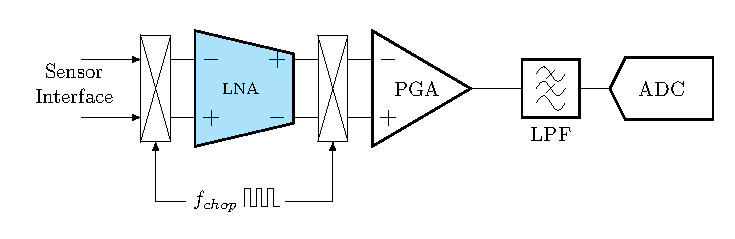
\includegraphics[ width = 0.9\columnwidth]{img/sensor-interface.pdf} 
    \caption{ A typical bio-sensing AFE.}
    \label{fig:sensor interface}
\end{figure}

\subsection{CCIA Design Equations}

% \begin{figure}[!h]
%     \begin{subfigure}[c]{0.49\linewidth}
%       \begin{subfigure}[t]{\textwidth}
%         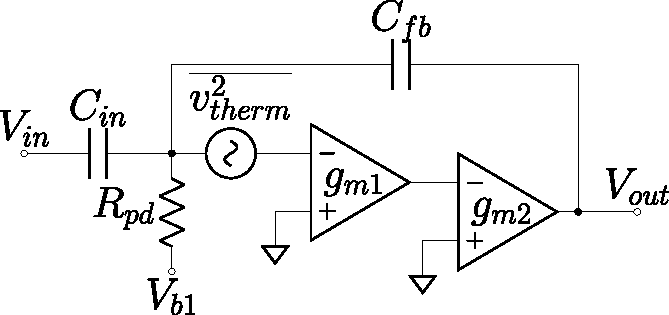
\includegraphics[width=\textwidth]{img/CCIA.pdf}
%         \label{fig:CCIA}
%         \caption{}
%       \end{subfigure}
%       % NOTE2: two empty lines = 1 linebreak

%       \begin{subfigure}[c]{\linewidth}
%         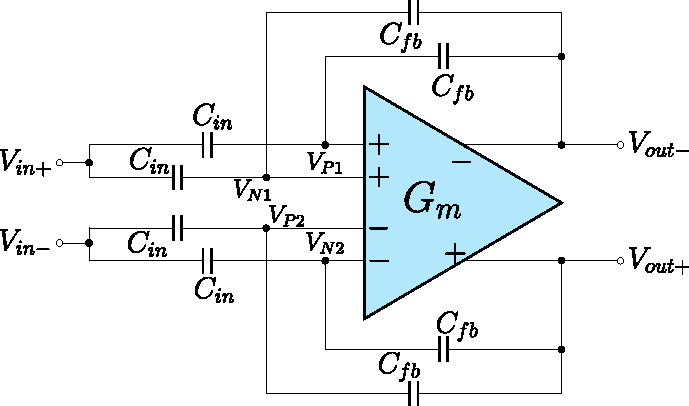
\includegraphics[width=\textwidth]{img/DL-CCIA.pdf}
%         \caption{}
%         \label{fig:DLCCIA}
%       \end{subfigure}
%     \end{subfigure}
%     \hfill  % NOTE1: hfill moves horizontally stacked objects as far apart as it can
%     \begin{subfigure}[c]{0.49\linewidth}
%       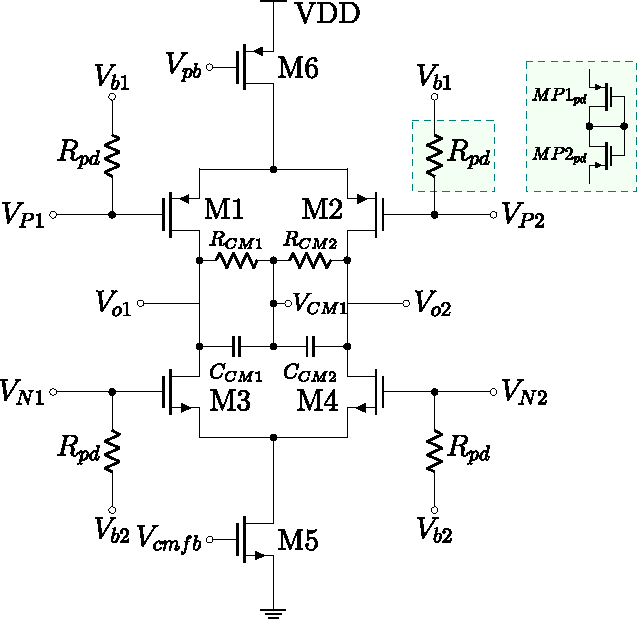
\includegraphics[width=\textwidth]{img/CurrentReuse.pdf}
%       \label{fig:CRCI}
%       \caption{}
%     \end{subfigure}
%     \caption{ (a) a CCIA implemented with two amplifier stages (b) CCIA schematic with dual-loop architecture (c) Current-reuse amplifier ($g_{m1}$) schematic}
%     \label{fig:CCIA and current reuse}
%   \end{figure}

\begin{figure}[!h]
       \centering
       \begin{subfigure}[c]{0.49\linewidth}
           \centering
           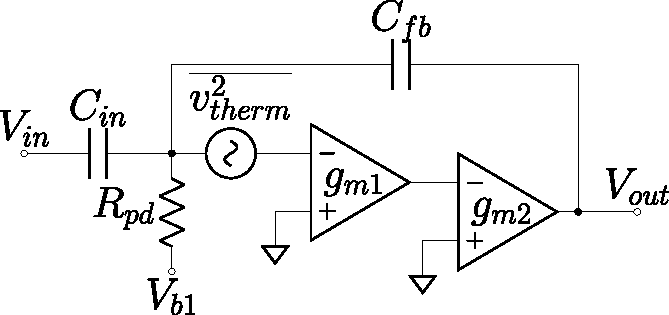
\includegraphics[width=\linewidth]{img/CCIA.pdf}
           \caption[]%
           {{\small }}
           \label{fig:CCIA}
        \end{subfigure}
        \hfill
        \begin{subfigure}[c]{0.49\linewidth}  
            \centering 
            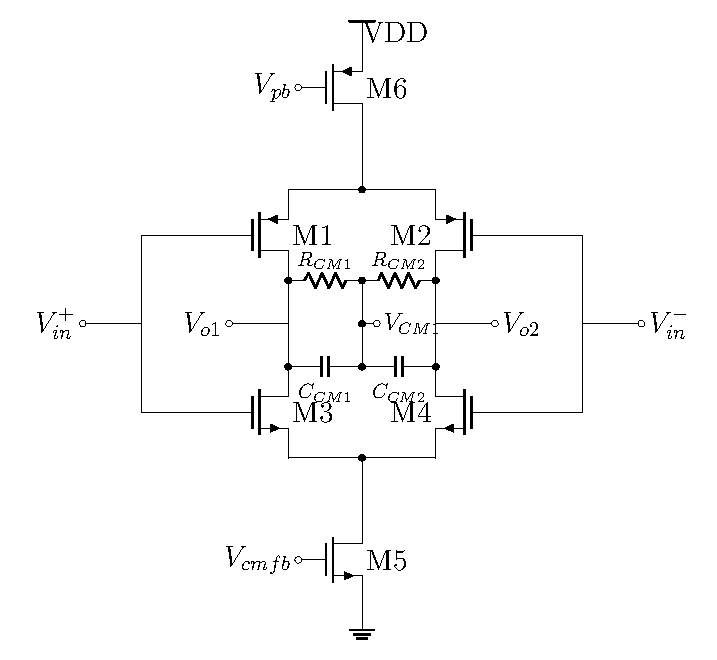
\includegraphics[width=\linewidth]{img/CurrentReuseSharedBias.pdf}
            %\caption[5 DOF custom mount for MPFCS]%
            %{{\small 5 DOF custom mount for MPFCS}}    
            \caption[]%
            {{\small }}
            \label{fig:CRCISHAREDBIAS}
        \end{subfigure}
        \caption[ Don't write caption here ]
        {\small (a) CCIA implemented with two amplifier stages (b) Current-reuse amplifier ($g_{m1}$) schematic. } 
        \label{fig:CCIA and current reuse}
\end{figure}

%\begin{figure} [!htbp]
%   \centering
%    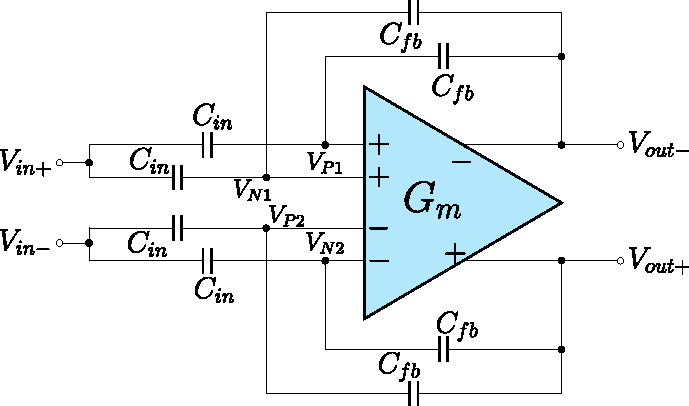
\includegraphics[width = 0.65\linewidth]{img/DL-CCIA.pdf}
%    \caption{ CCIA schematic with dual-loop architecture.}
%    \label{DLCCIA}
%\end{figure}

%The small signal gain of the CRCI is given by:

% \begin{equation}
%     A_{g_{m,1}} = \left(\left(\frac{g_m}{I_D} \right)_P + \left(\frac{g_m}{I_D} \right)_N\right)/\left(\left(\frac{g_{ds}}{I_D} \right)_P+\left(\frac{g_{ds}}{I_D} \right)_N\right) \label{eq:small signal gain}
% \end{equation}

To reduce thermal noise in the MOSFET, the current reuse complementary input (CRCI) topology depicted in \cref{fig:CRCISHAREDBIAS} was implemented. The advantage of this topology is a doubling of the input transconductance without increasing the bias current, allowing the input-referred thermal noise ($v_{therm}$) to be reduced by a factor of $\sqrt{2}$. Modelling $v_{therm}$ of the differential structure referred to its negative input yields:

{\small
\begin{equation}
    v_{therm} \approx \sqrt{\frac{8 k_B T\gamma}{I_{D} \left(\left( \frac{g_m}{I_D} \right)_P+\left(\frac{g_m}{I_D} \right)_N \right) }}\label{eq:vinamp}
\end{equation}
}%
where $k_B$ is Boltzmann constant, $T$ is temperature (in Kelvin), $\gamma$ is the Mosfet noise coefficient, $I_D$ is the device bias current, and $\left(\frac{g_m}{I_D}\right)_{P,N}$ is the transconductance efficiency of M1,2 and M3,4 respectively (see \cref{fig:CRCISHAREDBIAS}).

The total noise at the LNA input is the input-referred noise (IRN) of the CCIA ($v_{in,ref}$) plus the output noise from the electrode or sensor capturing the Bio-signal $\overline{v_{n,sensor}^2}$. The total noise is given by:

{\footnotesize
\begin{align}
\overline{v_{in,ref}^2} &= \left(\underbrace{(C_{in} + C_{g} + C_{fb})/C_{in}}_{\eta\text{: Noise Gain Factor }}\right)^2\left(\overline{v_{f_c}^2} + \overline{v_{therm}^2}\right) + \overline{v_{n,sensor}^2} \label{eq:system_noise}
\end{align}
}%

where $C_g$ is the input parasitic capacitance, $C_{in}$ is the CCIA input capacitance, $C_{fb}$ is the CCIA feedback capacitance, and $\overline{v_{f_c}^2}$ is the LNA flicker noise.

\subsection{Chopping, Settling and Frequency Planning}

Chopping is a popular technique used to reduce flicker noise, but requires careful consideration of amplifier settling time and frequency planning. \Cref{fig:without-chopping} and \Cref{fig:chopping} depict the frequency spectrum without chopping and with chopping enabled. The requirement to keep the flicker noise out of the signal bandwidth, such that the signal bandwidth $f_{sig} < f_{chop} - f_{c}$. $f_{c}$ is the flicker noise corner, and $f_{chop}$ is the chopping frequency. Adding chopping requires the CCIA to settle after switching events.

\begin{figure}[!h]
        \centering
        \begin{subfigure}[c]{0.45\linewidth}
            \centering
            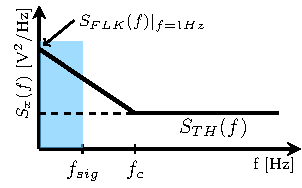
\includegraphics[width=\linewidth]{img/without-chopping-spectrum.pdf}
            \caption[]%
            {{\small }}
            \label{fig:without-chopping}
        \end{subfigure}
        \hfill
        \begin{subfigure}[c]{0.45\linewidth}  
            \centering 
            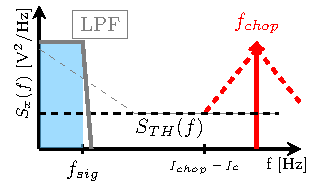
\includegraphics[width=\linewidth]{img/chopping-spectrum.pdf}
            \caption[]%
            {{\small }}
            \label{fig:chopping}
        \end{subfigure}
        \caption[ Don't write caption here ]
        {\small (a) Spectrum without chopping (b) Spectrum with chopping} 
        \label{fig:with-chopping}
\end{figure}
The settling time ($T_{settle}$) of the CCIA is constrained by the resolution ($N$) of the ADC conversion, $f_u$, the CCIA unity gain bandwidth, and $\beta=C_{fb}/(C_{in} + C_{fb} + C_g)$:
% {\small
\begin{equation}
    T_{settle} = \frac{1}{\beta 2 \pi f_u} \ln \left( \frac{1}{2^N} \right) \label{eq:Settle_time}
\end{equation}
% }%
As a prudent measure $T_{settle} < \frac{1}{2}\frac{1}{f_{chop}}$.
